
\section{Training the models} % ----------------------------------------------
In order to train our custom ResNet CNN, the SGD optimizer was used with mostly the same HPs as the original paper, minus the learning rate, which is two orders of magnitude smaller due to the fact that our network is shallower than the original one. The loss function is MSE, and the SGD HPs used for training are:
\begin{itemize}
    \item \textbf{Learning rate:} $\eta =1\times 10^{-3}$, with a plateau decaying factor of 0.2, meaning that if during training the validation loss becomes stationary, the LR is reduced to allow for finer gradient steps necessary for converging to a local minima.
    \item \textbf{Momentum:} $\beta = 0.9$, which applies gradient smoothing using a weighted moving average on the succession of gradients. Formally:
    \begin{equation*}
    \centering
        \begin{gathered}
        m_t = \beta m_{t-1} + (1-\beta)\nabla L(W_t)  \\
        W_{t+1} = W_t - \eta_t m_t\\
        \end{gathered}
    \end{equation*}
    Where $m_t$ is the gradient computed at time $t$, $W_t$ are the weights of the network, $\nabla L$ is the loss gradient (computed wrt. a random extraction of one datapoint), $\eta_t$ is the learning rate, and $\beta$ is the momentum.
    \item \textbf{Weight Decay:} $\lambda =1\times10^{-4}$, is a regularization technique which consists in adding to the loss a penalty term proportional to the L2 norm of the weights in the network.\\
    Putting it all together, the penalty term and final weight update become:
    \begin{equation*}
    \centering
        \begin{gathered}
        L_{\lambda}(W) = L(W) + \frac{\lambda}{2}||W||^2  \\
        W_{t+1} = W_t - \eta_t (m_t +\lambda W_t)\\
        \end{gathered}
    \end{equation*}
     
\end{itemize}

\noindent
Apart from the ResNet training, all subsequent training runs have been performed using the \textit{Adam} \cite{kingma2014adam} optimizer and MSE as the loss function.

\textit{Adam} combines the momentum technique described above, with \textit{RMSProp}, which is a similar technique but considers the weighted moving average of the squared gradients, which approximates the gradients variance:
    $$
        V_t = \gamma V_{t-1} + (1-\gamma)(\nabla L(W_t, X_t, Y_t))^2  
    $$
Then uses the squared root of this moving average to adaptively reduce the learning rate. Thus, the update rule for the weights becomes:
    $$
        W_t = W_{t-1} - \frac{\eta_t m_t}{\sqrt{V_t + \epsilon}}
    $$
This ensures that each weight of the network is adjusted adaptively, with momentum smoothing and scaled updates in case of large gradients\footnote{The additional bias correction steps for the $m_t$ and $V_t$ terms were omitted for brevity.}. The stopping criterion for each run was EarlyStopping, with a patience of 7 epochs, and after stopping the training process, the best weights (i.e., those that minimize validation loss) are restored and saved to disk.

\subsection{Training results}
\noindent
After having optimized each model, a training run is performed with the best HPs and $k$-fold cross validation is used to obtain robust estimates for the model performances. The results are summarized in \textbf{Table \ref{tab:perf_comparison}}, whereas \textbf{Figure \ref{fig:train_perf}} shows the training loss and validation loss curves observed during training. 


\begin{table}[ht!]
    \centering
    \newcolumntype{Y}{>{\centering\arraybackslash}X}
    \begin{tabularx}{\textwidth}{YYYYY}
        \hline
        \textbf{Model}       & \textbf{Train Loss} & \textbf{Val Loss} & \textbf{Test Loss} & \textbf{5-fold CV}\\
            \hline 
            \textbf{ResNet}       &  &  &  & \\
            Baseline        & 0.0368      & 0.0365              & 0.0354            & 0.0416\\ 
            Optimized       & 0.0366      & \bt{0.0358}         & \bt{0.0352}       & \bt{0.0367}\\ 
             \hline
             
            \textbf{EfficientNet}       &  &  & & \\
            Baseline        & 0.0355      & 0.0370              & 0.0364            & 0.0382 \\ 
            Optimized       & 0.0351      & 0.0361              & 0.0363            & 0.0376 \\ 
             \hline
             
            \textbf{MobileNet}          &  &  & & \\
            Baseline        & 0.0261      & 0.0417              & 0.0452            & 0.0471 \\ 
            Optimized       & 0.0359      & 0.0362              & 0.0356            & 0.0519 \\ \hline
    \end{tabularx}
    \captionof{table}{Baseline vs optimized performance of the three CNNs.}
    \label{tab:perf_comparison}
\end{table}

\noindent
Finally, the number of parameters and the inference time of the optimized models are summarized in \textbf{Table \ref{tab:inference_times}}, where the GPU used for these tests is an RTX2080 and the CPU an i7-9700K. The inference times reported are relative to a single datapoint; calculated by dividing the inference time of a batch by its cardinality.
\begin{table}[ht!]
    \centering
    \newcolumntype{Y}{>{\centering\arraybackslash}X}
    \begin{tabularx}{\textwidth}{YYYYY}
        \hline
        \textbf{Model}              & \textbf{Tail params}  & \textbf{Head params} & \textbf{t-GPU(ms)} & \textbf{t-CPU(ms)}\\
            \hline 
            \textbf{ResNet}         & \num{389760}          & \num{135170}      & 0.6  & 4.2 \\ 
            \textbf{EfficientNet}   & \num{12930622}        & \num{1511170}     & 15.2 & 562  \\ 
            \textbf{MobileNet}      & \num{2996352}         & \num{542274}      & 4.5  & 250  \\ \hline
    \end{tabularx}
    \captionof{table}{Parameters count and inference time of each optimized model.}
    \label{tab:inference_times}
\end{table}



\begin{figure}[ht!]
    \centering
        \subfloat[Baseline ResNet]{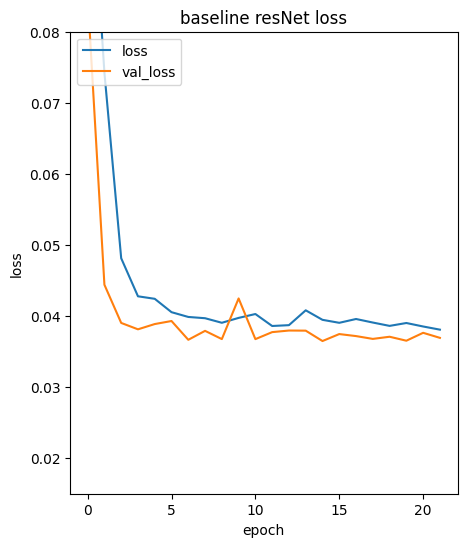
\includegraphics[height=.45\linewidth]{images/res_base.png}}\hspace{1cm}
        \subfloat[Optimized ResNet]{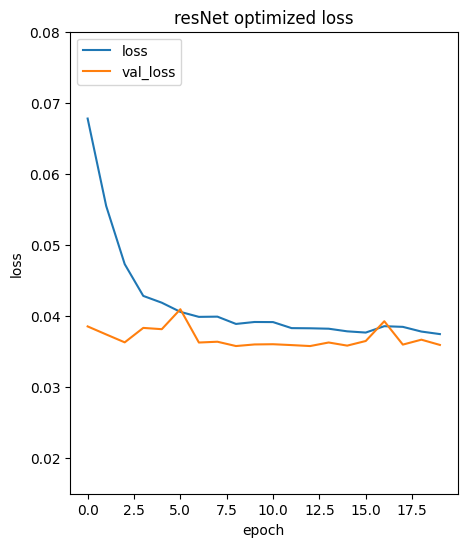
\includegraphics[height=.45\linewidth]{images/res_opt.png}}\hfill
        \subfloat[Baseline EfficientNet]{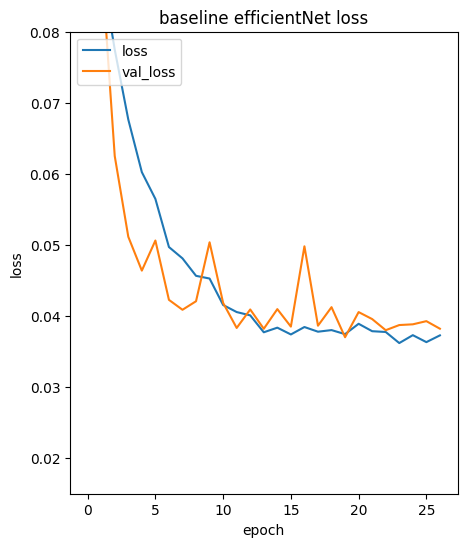
\includegraphics[height=.45\linewidth]{images/eff_base.png}}\hspace{1cm}
        \subfloat[Optimized EfficientNet]{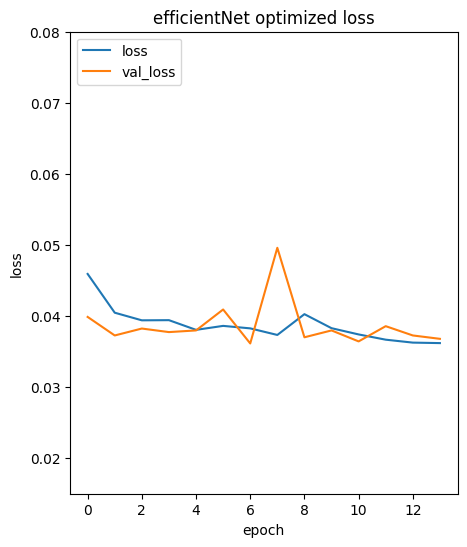
\includegraphics[height=.45\linewidth]{images/eff_opt.png}}\hfill
        \subfloat[Baseline MobileNet]{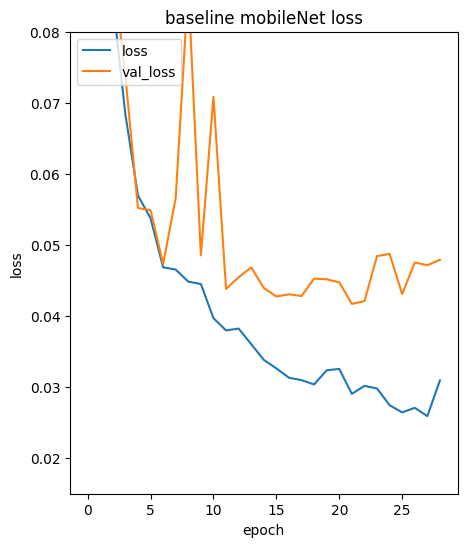
\includegraphics[height=.45\linewidth]{images/mob_base.png}}\hspace{1cm}
        \subfloat[Optimized MobileNet]{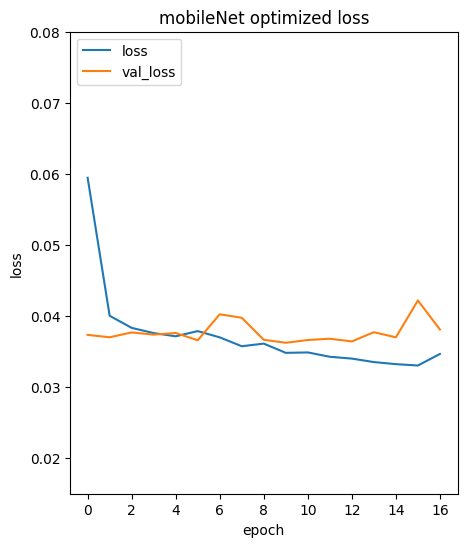
\includegraphics[height=.45\linewidth]{images/mob_opt.png}}
    \caption{Training curves of the various models}\label{fig:train_perf}
\end{figure}

\newpage